\chapter{Vergleich AOT vs. JIT}

\section{Programmausführung in der VM} \label{jit_vm}
Durch die Dynamik einer Programmiersprache, zur Schaffung einer Plattformunabhängigkeit oder aus Sicherheitsgründen werden Programme heutzutage oftmals nicht mehr direkt vom Betriebssystem ausgeführt, sondern laufen in einer \ac{VM}, wie dies bereits bei Smaltalk-80 der Fall war. Dies verzögert jedoch die Ausführungszeit der Interpretation der Befehle. \\
Durch die Anwendung von \ac{JIT} wird hier versucht Performance zu gewinnen und somit diesen Nachteil auszugleichen. Folgend sollen die beiden \ac{VM}'s 'HotSpot' und 'Graal' aus dem Kontext der Sprache Java näher vorgestellt werden. 

\subsection{HotSpot}
Java übersetzt den Code der Hochsprache generell zuerst in Bytecode, der in der \ac{VM} ausgeführt werden kann. Diese \ac{VM} wird speziell für das korrespondierende \ac{OS} bereitgestellt und kann auf dieser Plattform den erzeugten Bytecode korrekt ausführen. 'HotSpot' von Oracle ist eine dieser \ac{VM}'s für die Sprache Java. \\
\\
\begin{figure}[ht]
    \begin{center}
        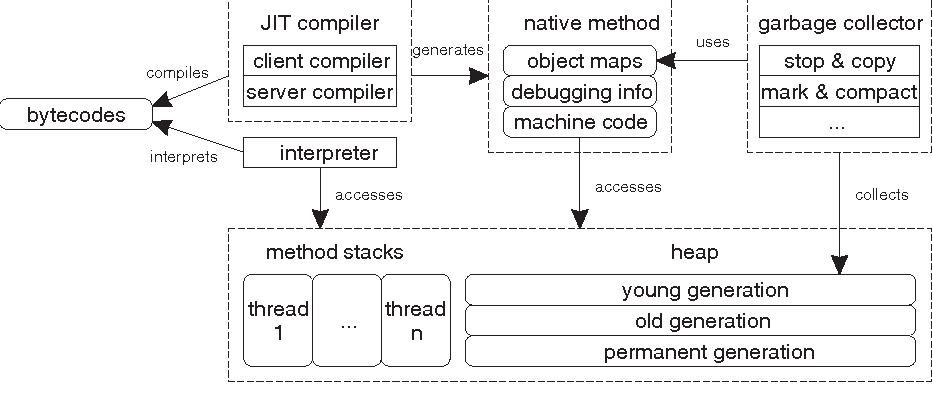
\includegraphics[width=0.9\textwidth]{assets/img/3-Figure1-1.png}
        \caption{Architektur 'HotSpot', \cite[Quelle: Kotzmann Wimmer 2008]{KotzmannWimmer2008}}
        \label{arch_hotspot}
    \end{center}
\end{figure}
Wie in \autoref{arch_hotspot} zu sehen, beginnt die Ausführung in der 'HotSpot'-\ac{VM} beim Interpreter. Hier wird der Bytecode schrittweise ausgeführt anhand von Templates ausgeführt. Nur die heuristisch am meisten frequentierten Codeblöcke werden durch den \ac{JIT}-Compiler kompiliert.\\
Wird während der Ausführung eine besonders aufwändige Schleife entdeckt, so wird diese ebenfalls kompiliert und die Ausführung dafür gestoppt. Die Schwierigkeit besteht hierbei darin, dass die Ausführung zwischen Interpreter und dem kompilierten Code synchronisiert werden muss. Dafür wird ein neuer Stackframe erstellt und initialisiert. Die Ausführung der Methode geht im nativen Code weiter. Dieses Verfahren nennt man \ac{OSR}.\\
'HotSpot' enthält zwei verschiedene Compiler, die für Server- und Clientsysteme gedacht sind. Bei Serversystemen wird sehr großer Wert auf eine sehr gute Optimierung gelegt, dafür jedoch eine längere Kompilierungszeit in Kauf genommen. Für dauerhaft laufende Serveranwendungen geht man davon aus, dass bereits während der Anlaufphase der Software der \ac{JIT}-Compiler alle wichtigen Methoden und Blöcke kompiliert und optimiert. Die längere Zeit ist hierfür nicht relevant, da die einmal kompilierten Sequenzen danach während der ganzen Laufzeit der Software zu Verfügung stehen.\\
Der Compiler für die Clientsysteme zielt auf Programme mit \ac{GUI} ab. Hier wird der Fokus auf die Antwortzeit der Oberfläche und damit den Punkt \ac{UX} gelegt. Dazu ist der \ac{JIT}-Compiler auf eine schnelle Kompilierung statt Performance ausgelegt.\\
Reservierter Speicher wird in drei Bereichen verwaltet. Neu kompilierte Methoden werden zuerst im Bereich der 'Young Generation' abgelegt. Füllt sich dieser Bereich, wird eine 'stop-and-copy' \ac{GC} initialisiert. Diese prüft, ob ein Objekt noch in Benutzung ist und löscht alle übrigen, um Speicher wieder freizugeben. Übersteht eine Methode mehrere Runden, wird sie in den Bereich der 'Old Generation' übernommen. Der Dritte Bereich wird als 'Permanent Generation' bezeichnet und enthält interne Datenstrukturen. Dieses Schema ist in \autoref{arch_hotspot} dargestellt, \cite[vgl. Kotzmann und Wimmer 2008, S.3f]{KotzmannWimmer2008}.\\

\subsection{GraalVM}
Die GraalVM ist ein System, das die \ac{VM} HotSpot ergänzen soll und dazu ein breites Subsystem an Tools für mehr Flexibilität mitbringt (siehe \autoref{arch_graal}). Graal zeichnet sich dadurch aus, dass es komplett selbst in Java geschrieben ist. \\
\\
\begin{figure}[ht]
    \begin{center}
        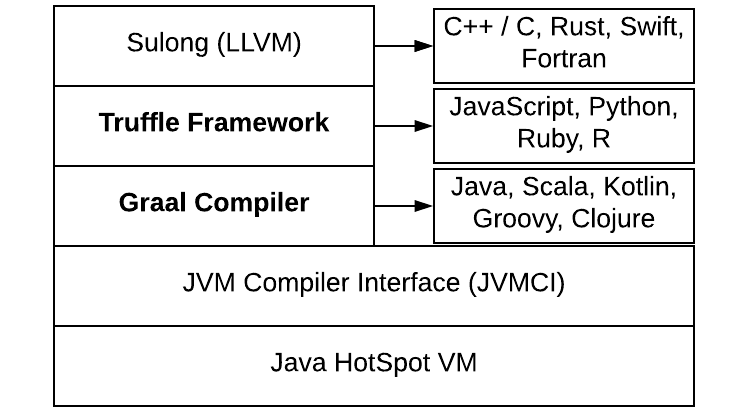
\includegraphics[width=0.9\textwidth]{assets/img/GraalVM-Architecture.png}
        \caption{Architektur 'HotSpot', \cite[Quelle: Sipek 2020]{Sipek_2020}}
        \label{arch_graal}
    \end{center}
\end{figure}
GraalVM setzt an der HotSpot \ac{VM} an und nutzt alle HotSpot Komponenten, die nicht direkt in den Prozess der Kompilierung eingebunden sind. Diese Kompilierungstools stellt Graal selbst zur Verfügung und wird über die \ac{JVMCI} mit der HotSpot \ac{VM} verbunden. \\
Die Motivation für den Tausch des Compilers oberhalb der \ac{VM} liegt in dessen Vielfältigkeit. Wie in \autoref{arch_graal} zu sehen bringt der Graal-Compiler ein breites Subsystem mit, dass eine Anwendung sehr viel flexibler machen kann. Der integrierte Graal Compiler unterstützt \ac{JVM} basierte Sprachen, wie Java, Scala, Kotlin, Groovy oder Clojure und kann somit als generalisierter \ac{JIT} Compiler für eine breite Plattform an Sprachen eingesetzt werden. Dies macht es für Entwickler wesentlich einfacher in den genannten Sprachen zu entwickeln, wenn sie bereits mit der zugrunde liegenden Technik von HotSpot vertraut sind. Ein Wechsel des Technik-Stacks entfällt und ein Einstieg in neue Sprachen fällt ungemein leichter. \\
Neben der Funktion als \ac{JIT}-Compiler bringt Graal auch die Möglichkeit mit, native Images zu erstellen und somit den Ansatz des \ac{AOT} zu erfüllen. Dieses Feature wird in \autoref{graal_aot} näher beleuchtet.\\
Das in \autoref{arch_graal} noch ersichtliche Truffle-Framework führt einen ähnlichen Ansatz, wie bereits der in Graal integrierte Compiler und erweitert die \ac{VM} für den Support weiterer Sprachen, wie z.B. JavaScript, Python, Ruby oder R. Truffle nutzt einen \ac{AST}, um den Code zu interpretieren und auszuführen. Dies stellt einen sehr einfachen Weg dar, kostet aber Ressourcen und kann z.T. in einer schwachen Performance resultieren. Graal setzt hier an und kann erzeugte \ac{AST} in hochoptimierte native ausführbare Dateien kompilieren. Um Overhead einzusparen kann dabei eine beliebige Anzahl \ac{AST} verbunden werden und als ein einziger interpretiert werden.\\
Über Truffle steht noch die Compiler-Infrastruktur-Engine 'Sulong', die Bitcode aus Low-Level Sprachen, wie z.B. C, C++, Fortan, Rust oder Swift, interpretieren kann. Das erweitert das Einsatzspektrum der GraalVM nochmals stark und es kann nahezu das ganze Feld der bekannten Sprachen eingesetzt werden \cite[vgl. Sipek 2020, S.2]{Sipek_2020}
\subsubsection{Native Image: Graal als AOT-Compiler} \label{graal_aot}

\section{Optimierung/Profiling}
